\section{Simulator}
\label{sec:PoC-Simulator}
\index{PoC!Simulator}

\begin{figure}[t]
  \centering
  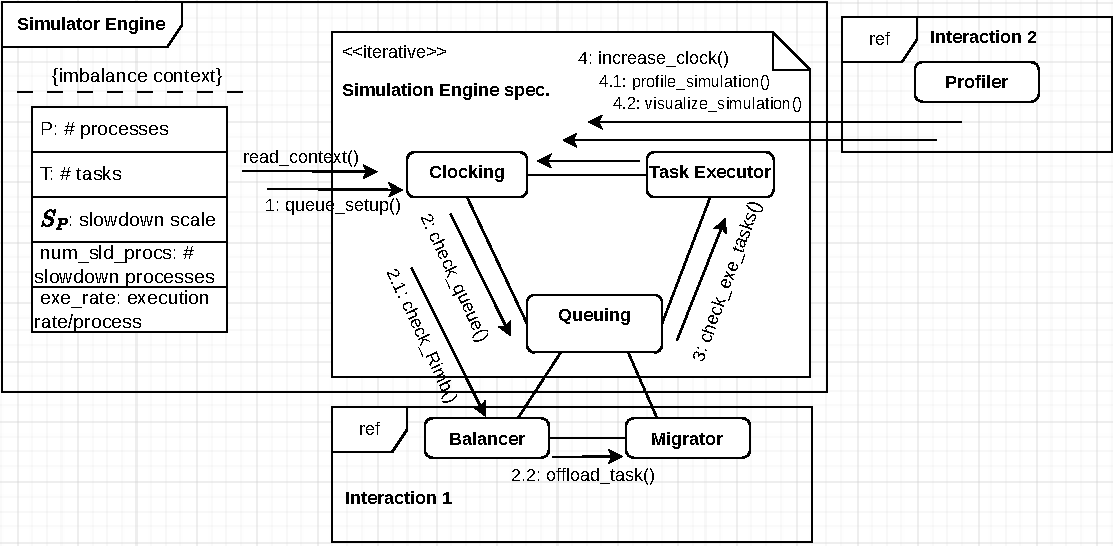
\includegraphics[scale=0.7]{./pictures/poc_implementation/poc_simulator_comm_diagram.pdf}
	\caption{A customed communication diagram of dynamic load balancing simulation.}
	\label{fig:simulator_comm_diagram}
\end{figure}

Following the design shown in Figure \ref{fig:react_lb_simulator}, we present in this section more about how its modules communicate as well as how we implement the simulator. Figure \ref{fig:simulator_comm_diagram} shows a customed communication diagram of the simulator's modules. The main frame indicates our simulator engine. On the left are the constraints we can also consider as input for simulation. We have these constraints to declaring imbalance context based on the number of involved processes ($P$), tasks ($T$), the scale of slowdowns such as $20\%$, $30\%$, or $50\%$, ..., then the number of processes being slow. The last input is the execution rate which denotes how many tasks can be done per time unit, or we can say how the throughput of execution (tasks/time unit) is.\\

Along with time units in clocking, this value can be adjusted for the ratio between the overhead of task migration, balancing operations, and time-step clocking. Next to the constraint block is a specification region of the simulator engine. Its behavior is iterative based on clocking. There are three modules:
\begin{itemize}
	\item \textbf{Clocking}: configures and manage time steps counting. It is associated with \textbf{Queuing} and \textbf{Task Executor}.
	\item \textbf{Queuing}: manages task distribution on processes. The constraint input determines each process's queue. In the beginning, the action \texttt{read\_context()} employs queuing tasks, and their execution time ($w$) setting relies on the given constraints.
	\item \textbf{Task Executor}: takes tasks from the queues and emulates the execution in parallel. This means at a time step, all queues are checked. Tasks are executed slow or fast based on the \texttt{exe\_rate}.
\end{itemize}

Below the \texttt{Simulation Engine spec.} region is an iteraction region, including \texttt{Balancer} and \texttt{Migrator}. Each time clocking, the balancer will check the queue's status for imbalance ratio ($R_{imb}$). If $R_{imb}$ meets the requirement of offloading tasks, it will signal \texttt{Migrator} for further actions to offloading tasks. Additionally, there is the second interaction region named \texttt{Profiler}. Before a time clock is closed, we can trigger the profiler to trace and record data for visualizing the simulation of our execution with dynamic load balancing. As we can see, the diagram extends the design in Figure \ref{fig:react_lb_simulator} to a communication diagram in more detail. Following the action arrows, we can determine the working flow from the points of simulation view. For example, after getting the imbalance context, we start with \texttt{queue\_setup()}, and \texttt{Clocking} is managed to proceed. Then, the behavior contineou by checking the queues (\texttt{check\_queue()}), ... until the termination of a loop (at \texttt{4.} \texttt{increase} \texttt{\_clock()}).\\

\begin{figure}[t]
  \centering
  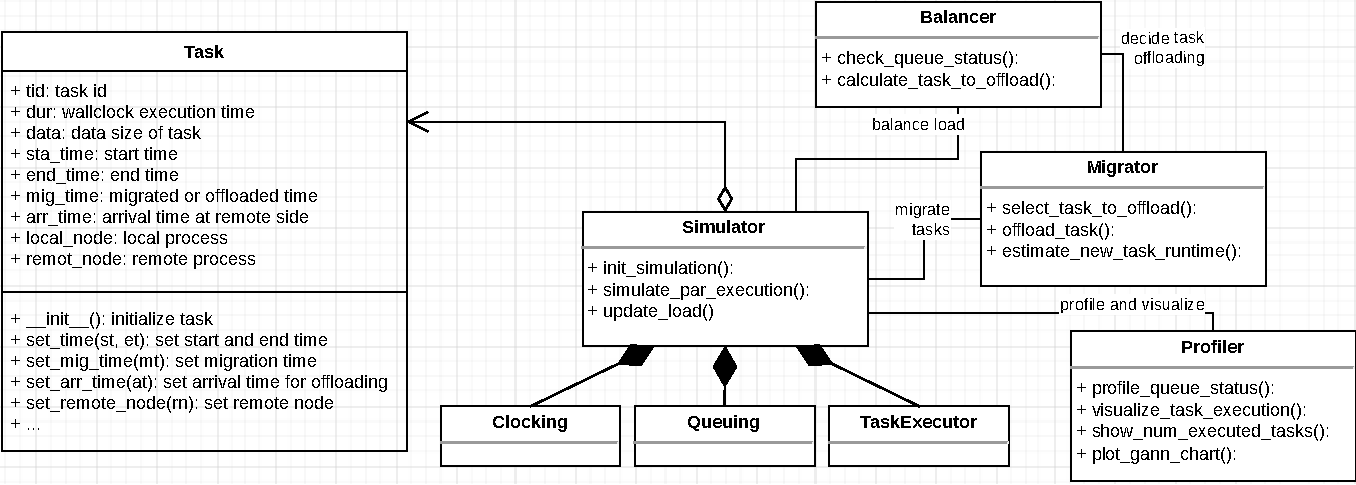
\includegraphics[scale=0.65]{./pictures/poc_implementation/poc_simulator_class_diagram.pdf}
	\caption{A class diagram of dynamic load balancing simulator.}
	\label{fig:simulator_class_diagram}
\end{figure}

Look into more detail, Figure \ref{fig:simulator_class_diagram} shows a class diagram of the simulator. Regarding task model, we show what the relevant properties to manage tasks during execution and balancing are. The task's properties consist of a unique id (\texttt{tid}), wallclock execution time (\texttt{dur}), and other important attributes related to time such as start time (\texttt{sta\_time}), end time (\texttt{end\_time}), migrated/offloaded time (\texttt{mig\_time}), etc. Behind the properties are their methods for setting or getting the corresponding values, e.g., \texttt{set\_time(st, et)} to set ``start'' and ``end'' time of a task, \texttt{set\_mig\_time(mt)} to set ``migrated'' time if a task is selected for offloading. The main interface is \texttt{Simulator}, which has an aggregation link with class \texttt{Task}. Inside \texttt{Simulator}, there are three interfaces also mentioned in the communication component. To be strongly dependent on \texttt{Simulator}, the internal methods (\texttt{init\_simulation()}, \texttt{update\_load()}, ...) have a composition link with \texttt{Clocking}, \texttt{Queuing}, and \texttt{TaskExecutor}. The other association links with \texttt{Simulator} are \texttt{Balancer}, \texttt{Migrator}, and \texttt{Profiler}. The \texttt{Balancer} checks all queue's status over time steps (by a method \texttt{check\_queue\_status()}) to calculate the imbalance level among processes. If $R_{imb}$ satisfies our defined imbalance constant, then \texttt{calculate\_task\_to\_offload()} will be invoked to decide tasks for offloading. Associated with \texttt{Migrator}, our simulation engine goes into the methods, i.e., \texttt{select\_task\_to\_offload()}, \texttt{offload\_task()}, \texttt{estimate\_new\_task\_runtime()} to perform task migration from one process to another. In the scope of this module, the properties, called \texttt{mig\_time} and \texttt{arr\_time}, are updated to fit our specification about communication overhead like latency, delay. Eventually, \texttt{Profiler} is a support module to profile and visualize the execution behavior. Besides, it helps to conduct statistics about performance and imbalance ratio at the end.

\begin{shaded}
	\noindent \textbf{A simulation example with $8$ processes, $R_{imb} \approx 1.5$}
\end{shaded}

\noindent This example is intended to show how the simulator works in a specific imbalance context. We re-use a consistent case of $R_{imb} \approx 1.5$ with $8$ processes, where each rank is assigned $100$ uniform tasks. Below is an input sample that we put into the simulator.

\begin{lstlisting}[language=Python, caption={An input sample for simulator}, label={lst:sim_input_sample}]
	num_process: 8
	num_tasks:   800
	slowdown:    0.2 # the scale of slowdown
	num_sld_processes: 2 # the number of slowed processes
	bandwidth: 1485 MB/s # bandwidth value for calculating delay
	exe_rate: 1.0 task/s # the execution rate
\end{lstlisting}
\hfill

Such the input, we distributed equally $100$ tasks per rank. The simulation is set with time steps in milliseconds (ms), and the clock is counted one by one at a time. With the execution rate $1.0$ task/s, the total load value of each rank in an ideal case is $100$s. Nevertheless, the case is configured with $2$ slowed processes, where the slowdown scale is $0.2$. We basically select $P0$ and $P1$ to be the slowed ranks. Thus, the tasks executed on their side take longer, $5$s, instead of $1$s in other ranks. The completion time will be $500$s in total because of performance slowdown without dynamic load balancing.\\

\begin{figure}[t]
  \centering
  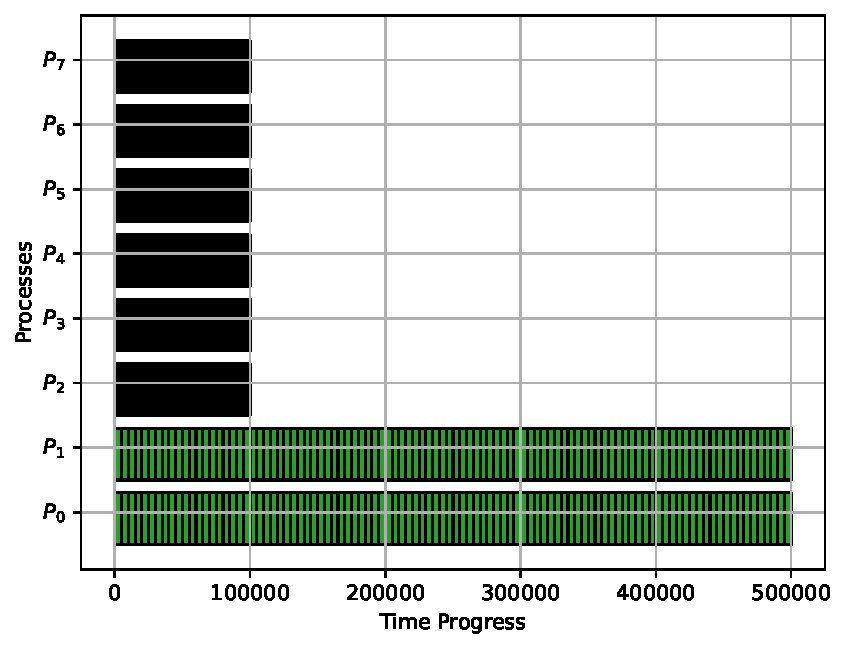
\includegraphics[scale=0.65]{./pictures/poc_implementation/poc_visualize_baseline_case_8_processes.pdf}
	\caption{A baseline case of simulation without dynamic load balancing.}
	\label{fig:simulator_baseline_case}
\end{figure}

Figure \ref{fig:simulator_baseline_case} shows the baseline case as described. The \texttt{Balancer} module is deactivated, and we can see the load imbalance of the baseline. The x-axis indicates the time progress direction of the execution; y-axis illustrates the load bars of $8$ processes. Green boxes denote executed tasks that are clearly seen at $P0$ $P1$. The load on other ranks compared to $P0$ and $P1$ is small; hence, we might see tasks on their sides as black. The following is a detailed output from our simulator (Listing \ref{lst:sim_output_sample}).

\begin{lstlisting}[language=Python, caption={The simulation output of the baseline case}, label={lst:sim_output_sample}]
-------------------------------------------
Configuration:
   + num. processes:     8
   + num. tasks:       800
   + slowdown:         0.2
   + num. sld.procs:     2
   + bandwidth:      1485.0 (MB/s)
   + exe_rate:         1.0 (task/s)
-------------------------------------------
----------------[PROFILING]----------------
	R0: num.local_tasks=  100, num.remote_tasks=    0
	R1: num.local_tasks=  100, num.remote_tasks=    0
	R2: num.local_tasks=  100, num.remote_tasks=    0
	R3: num.local_tasks=  100, num.remote_tasks=    0
	R4: num.local_tasks=  100, num.remote_tasks=    0
	R5: num.local_tasks=  100, num.remote_tasks=    0
	R6: num.local_tasks=  100, num.remote_tasks=    0
	R7: num.local_tasks=  100, num.remote_tasks=    0
----------------[PROFILING]----------------
	Write profiled queue data to: ./poc_visualize_baseline_case_8_procs_output.csv
-------------------------------------------
Simulation results:
-------------------------------------------
   + P[  0]: local_load= 500.00(s), remot_load=   0.00(s)
   + P[  1]: local_load= 500.00(s), remot_load=   0.00(s)
   + P[  2]: local_load= 100.00(s), remot_load=   0.00(s)
   + P[  3]: local_load= 100.00(s), remot_load=   0.00(s)
   + P[  4]: local_load= 100.00(s), remot_load=   0.00(s)
   + P[  5]: local_load= 100.00(s), remot_load=   0.00(s)
   + P[  6]: local_load= 100.00(s), remot_load=   0.00(s)
   + P[  7]: local_load= 100.00(s), remot_load=   0.00(s)
-------------------------------------------
Statistic:
-------------------------------------------
max. load:   500.0
min. load:   100.0
avg. load:   200.0
R_imb:         1.5
sum. overloaded_load:    600.0
sum. underloaded_load:   600.0
-------------------------------------------
\end{lstlisting}
\hfill

In case of applying reactive load balancing. We active the \texttt{Balancer} module and configure the simulator with balancing operation overhead and delay overhead when tasks are migrated at runtime. Also such a relax case, we try to set the balancing overhead $O_{\text{balancing}} = 1.0$ms and the delay for task migration $d=1$ms. In the fraction with task wallclock time units in seconds, we have a ratio of $1:1000$. Or we can say that the balancing overhead and delay time occupy $0.1\%$ of runtime unit.\\

\begin{figure}[t]
  \centering
  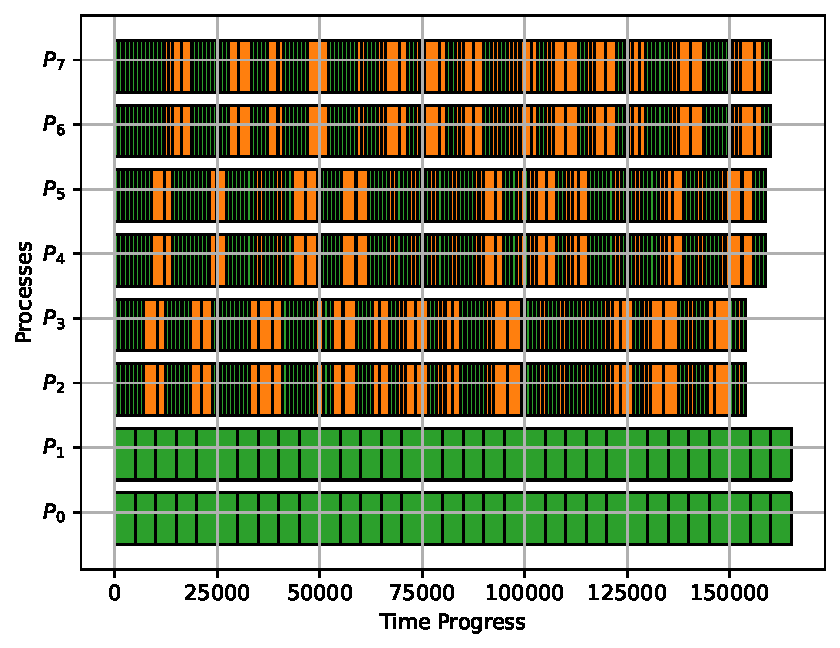
\includegraphics[scale=0.65]{./pictures/poc_implementation/poc_visualize_reactlb_O1_d1_8_processes.pdf}
	\caption{A reactive load balancing case of simulation with $O_{\text{balancing}} = 1.0$ms and $d=1$ms.}
	\label{fig:simulator_reactlb_O1_d1_case}
\end{figure}

Figure \ref{fig:simulator_reactlb_O1_d1_case} illustrates the simulation case with reactive load balancing, where $O_{\text{balancing}} = 1.0$ms and $d=1$ms. In overall, the completion time is reduced, where the orange region indicates remote tasks or offloaded tasks, the green region is local task execution. Wit $O_{\text{balancing}} = 1.0$ms and $d=1$ms, the simulator works as follows,
\begin{itemize}
	\item Assuming the current state at $t_{k}$, \texttt{Balancer} detects an imbalance and tasks from $P0$ should be offloaded to $P7$ as an example. However, the tasks are actually proceeded in the queue for offloading at $t_{k} + 1$.
	\item Similarly, assuming tasks from $P0$ are decided to offload to $P7$ at $t_{k}$. However, these tasks arrive at the $P7$ side at $t_{k} + 1$.
\end{itemize}

With this mechanism of clocks, we can postpone the procedure of dynamic load balancing to emulate it in practice. Listing \ref{lst:sim_output_reactlb_O1_d1} shows the output sample of this case applied reactive balancing approach. The maximum load, as well as completion time, is improved significantly $\approx 165.0$ms, and $R_{imb}$ is almost $0$ as an ideal case.

\begin{lstlisting}[language=Python, caption={The simulation output of reactive load balancing case with $O_{\text{balancing}} = 1.0$ms, $d=1$ms}, label={lst:sim_output_reactlb_O1_d1}]
-------------------------------------------
...
-------------------------------------------
----------------[PROFILING]----------------
	R0: num.local_tasks=   33, num.remote_tasks=    0
	R1: num.local_tasks=   33, num.remote_tasks=    0
	R2: num.local_tasks=   82, num.remote_tasks=   38
	R3: num.local_tasks=   82, num.remote_tasks=   38
	R4: num.local_tasks=   81, num.remote_tasks=   42
	R5: num.local_tasks=   81, num.remote_tasks=   42
	R6: num.local_tasks=   76, num.remote_tasks=   48
	R7: num.local_tasks=   76, num.remote_tasks=   48
----------------[PROFILING]----------------
	Write profiled queue data to: ./profiled_queues_reactlb_O1_d1.csv
-------------------------------------------
Simulation results:
-------------------------------------------
   + P[  0]: local_load= 165.00(s), remot_load=   0.00(s)
   + P[  1]: local_load= 165.00(s), remot_load=   0.00(s)
   + P[  2]: local_load=  82.00(s), remot_load=  72.50(s)
   + P[  3]: local_load=  82.00(s), remot_load=  72.50(s)
   + P[  4]: local_load=  81.00(s), remot_load=  75.00(s)
   + P[  5]: local_load=  81.00(s), remot_load=  75.00(s)
   + P[  6]: local_load=  76.00(s), remot_load=  81.00(s)
   + P[  7]: local_load=  76.00(s), remot_load=  81.00(s)
-------------------------------------------
Statistic:
-------------------------------------------
max. load:   165.0
min. load:   154.5
avg. load:   158.1
R_imb:         0.0
sum. overloaded_load:     13.8
sum. underloaded_load:    13.8
-------------------------------------------
\end{lstlisting}
\hfill

To see the visualization in detail with more significant overheads of balancing and task migration, we show the test cases of $d=2$ms and $O_{\text{balancing}}$ is $2, 5, 10, 20$ ms respectively, corresponding to the occupation of $0.2\%, 0.5\%, 1.0\%, 2.0\%$ over the runtime unit. Figure \ref{fig:simulator_reactlb_increased_O_d} shows these cases in visualized execution. Compared to the baseline and the relaxed case of $O_{\text{balancing}}$ $=1$ ms, $d=1$ ms, these figures highlight the impact of balancing overhead in reactive decisions on-the-fly. Not only delay time during task migration, the operations of load balancing, e.g., load monitoring, queue status exchange, and imbalance calculation, can affect the time we decide on tasks for offloading. This is sensitive and dependent on specific use cases of parallel applications. Such the case of $O_{\text{balancing}}$ occupying $0.5\%$ over task runtime, the balancing approach starts getting worse.

\begin{figure}[t]
\centering
\subfloat[Subfigure1][Reactive LB with $O_{\text{balancing}}$ $=2$ms and $d=2$ms]{
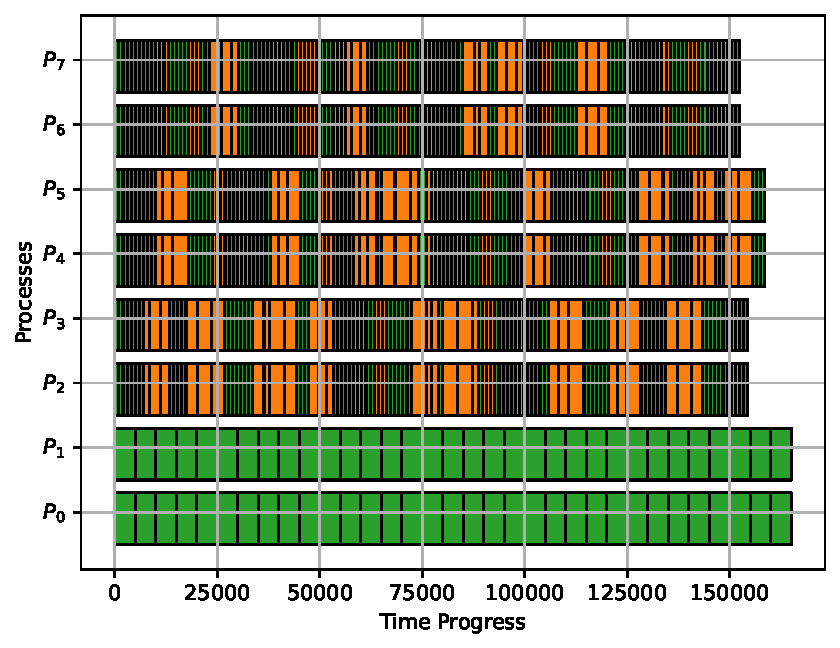
\includegraphics[scale=0.525]{./pictures/poc_implementation/poc_visualize_reactlb_O2_d2_8_processes.pdf}
\label{sfig:reactlb_O2_d2}}
\subfloat[Subfigure2][Reactive LB with $O_{\text{balancing}}$ $=5$ms and $d=2$ms]{
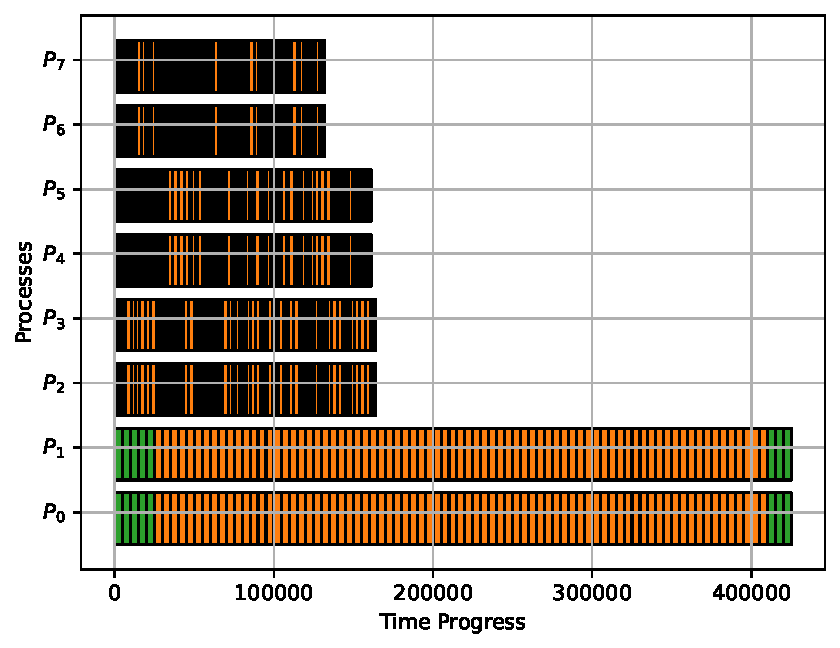
\includegraphics[scale=0.525]{./pictures/poc_implementation/poc_visualize_reactlb_O5_d2_8_processes.pdf}
\label{sfig:reactlb_O5_d2}}
\qquad
\subfloat[Subfigure3][Reactive LB with $O_{\text{balancing}}$ $=10$ms and $d=2$ms]{
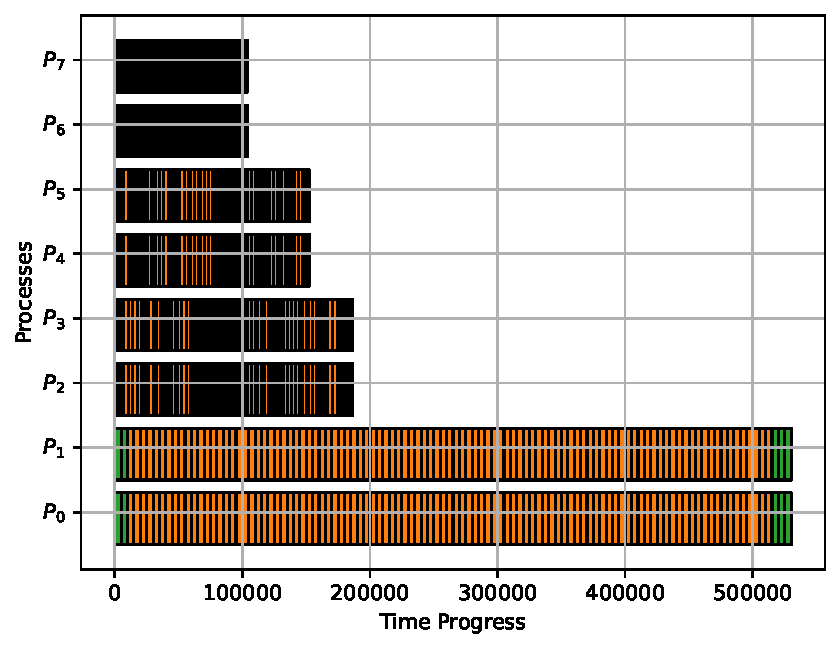
\includegraphics[scale=0.525]{./pictures/poc_implementation/poc_visualize_reactlb_O10_d2_8_processes.pdf}
\label{sfig:reactlb_O10_d2}}
\subfloat[Subfigure4][Reactive LB with $O_{\text{balancing}}$ $=20$ms and $d=2$ms]{
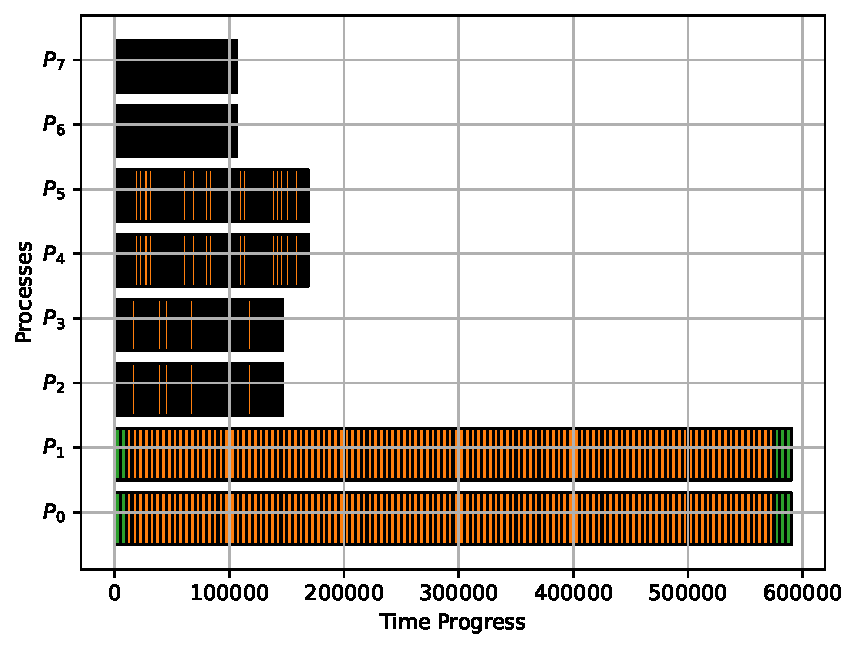
\includegraphics[scale=0.525]{./pictures/poc_implementation/poc_visualize_reactlb_O20_d2_8_processes.pdf}
\label{sfig:reactlb_O20_d2}}
\caption{A visualization of reactive load balancing with increased balancing overhead and delay.}
\label{fig:simulator_reactlb_increased_O_d}
\end{figure}